\chapter{Tools, Offsets and Tool Changes}
\label{ch:tools}

\section{The tool table}

\begin{figure}[H]
  \centering
  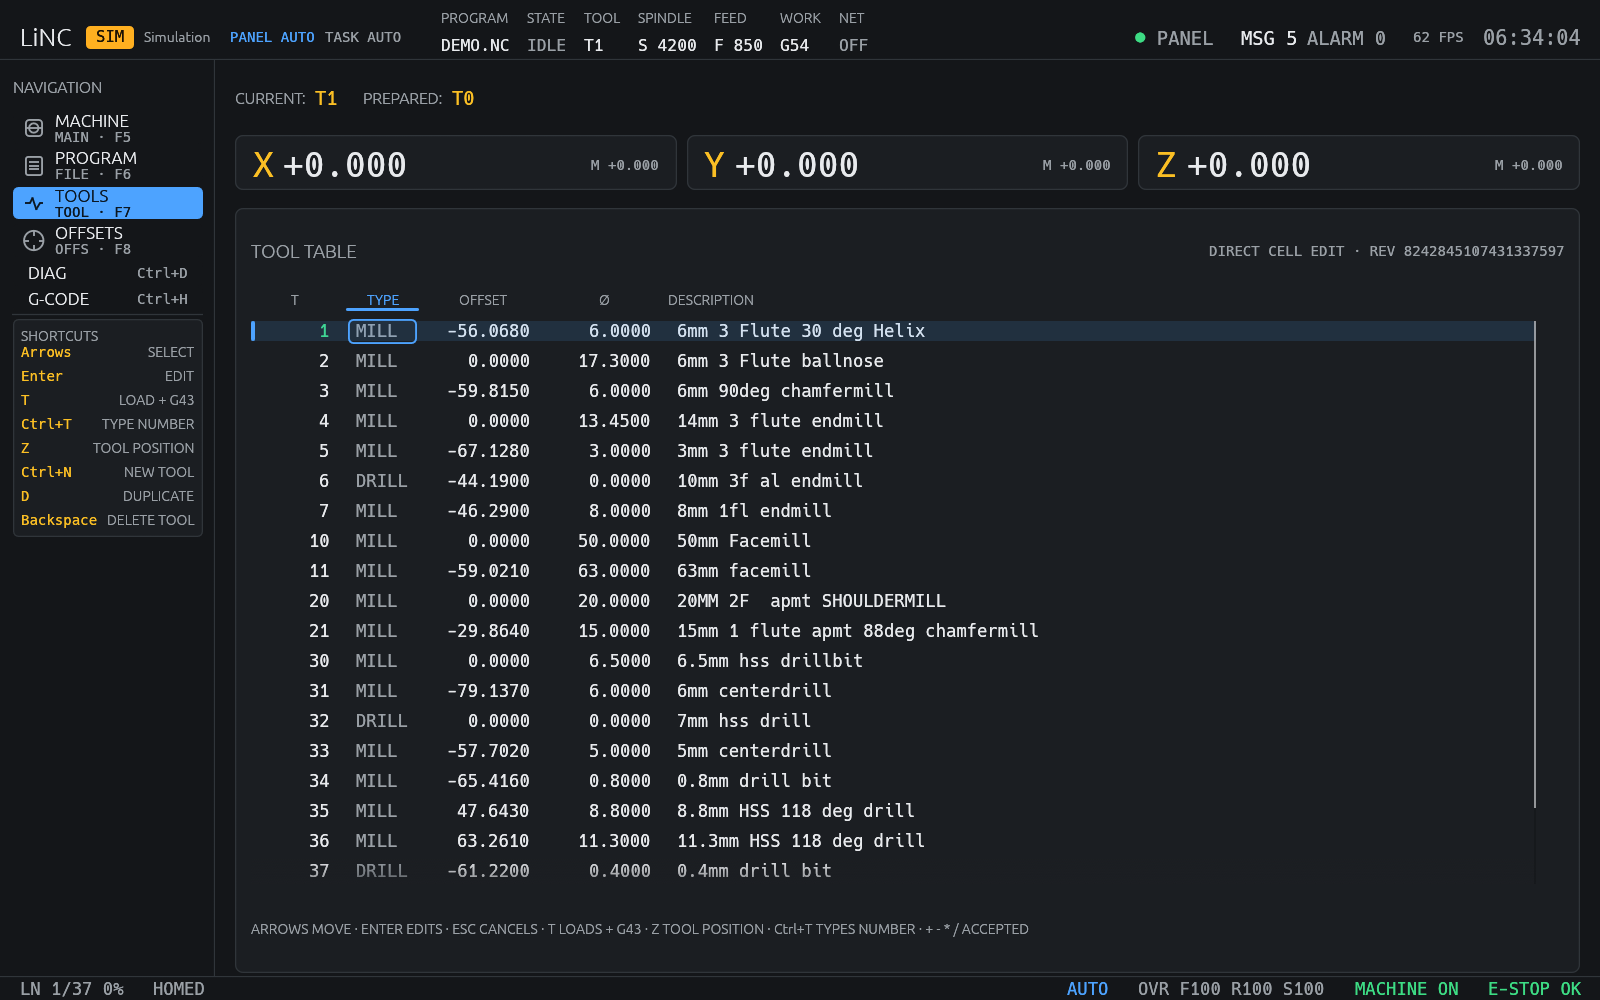
\includegraphics[width=\textwidth]{img/ui/tools.png}
  \caption{The Tools page. The table is the page: there is no separate change pane and no
           changer pane.}
  \label{fig:tools}
\end{figure}

The Tools page reads and writes the controller's standard tool table, the file named by
\texttt{[EMCIO] TOOL\_TABLE} in the machine INI. The columns come from the table's own
\texttt{TOOL\_TABLE\_COLUMNS}, so the page shows the schema the machine actually has.

Above the table, the current and prepared tools are named: \sbtn{CURRENT: T3},
\sbtn{PREPARED: T7}. A pocket column appears only on a machine with an automatic changer; a
manual-change machine hides it.

\begin{longtable}{L{3.2cm}L{9.6cm}}
  \toprule
  \textbf{Keys} & \textbf{Action} \\
  \midrule
  \endhead
  Arrows & Move through the table and its rows. The table takes the keyboard when the page
        opens. \\
  \keycap{Enter} & Edit the selected cell. The whole value is selected. \keycap{Enter} writes
        it; \keycap{Esc} restores the previous value. \\
  \keycap{T} & Load the selected row's tool: \texttt{Tn M6} and \texttt{G43 Hn} in one
        command, so length compensation is in effect when the change completes. \\
  \chordtwo{Ctrl}{T} & Type a tool number instead of cursoring to its row. \texttt{0}
        unloads the spindle. \\
  \keycap{Z} & Open the tool position dialog for the tool in the spindle. \\
  \chordtwo{Ctrl}{N} & Add a row with the next free tool number. \\
  \keycap{D} & Duplicate the selected row under the next free number. \\
  \keycap{Backspace} & Delete the selected row after a confirmation. \\
  \keycap{S} & Run one Loobric sync, when the machine has a Loobric server. \\
  \bottomrule
\end{longtable}

\begin{itemize}
  \item Writing a cell reloads the table into the controller and re-applies \texttt{G43} when
        the edited row is the tool in the spindle. The interface waits until the controller
        publishes the new row, so compensation cannot run against the table it is replacing.
  \item The probe tool and the tool in the spindle cannot be deleted, and the probe tool
        number is skipped when a new row is created.
  \item The `Z' column and the length field are one offset under two names: either cell writes
        both.
  \item An edited cell turns red while it holds an uncommitted value.
\end{itemize}

\section{The tool position dialog}

\keycap{Z} opens one line: \sbtn{SET <axis> POSITION}, the entry, and the offset the confirm
would write. It asks where the tool is now, seeded with the work coordinate the controller
reports, and writes the tool offset so the work coordinate reads the entered value.

\begin{itemize}
  \item \keycap{X}, \keycap{Y} and \keycap{Z} choose which coordinate is being entered.
  \item A \keycap{Z} entry updates the tool's length. \keycap{X} and \keycap{Y} update the
        geometry offsets the same way.
  \item The entry accepts arithmetic: \texttt{-12.5} and \texttt{10+2.5} both work.
  \item A refused write (machine off, running, protect, panel offline) keeps the dialog open
        and names the reason.
\end{itemize}

\section{Tool numbers without cursoring}

\chordtwo{Ctrl}{T} opens a one-line tool-number dialog, prefilled with the tool in the
spindle and fully selected, so \keycap{Enter} alone re-loads that tool.

Only a number the table carries, or \texttt{0}, is accepted. A refusal names the problem
(\texttt{T7 is not in the tool table}, an empty entry, a non-numeric one) and keeps the dialog
open.

\section{Manual tool changes}

On a machine with a manual changer, \texttt{M6} pauses for the change and a prompt appears --
on every page, not only on Tools:

\begin{description}[font=\normalfont\sffamily\bfseries, leftmargin=3.4cm, style=nextline]
  \item[\sbtn{INSTALL}] The tool to put in the spindle.
  \item[\sbtn{REMOVE}] The tool to take out, with its description.
  \item[\sbtn{CONFIRM}] The only action. It confirms that the tool is in.
\end{description}

The prompt follows the controller's request and cannot be dismissed. Confirming is a
handshake, not motion: it is allowed while the program is running or paused, and it does not
need cycle start. It raises the declared \halpin{linc.tool-change-confirm} output and holds it
until the controller drops its own request, so a short pulse cannot be missed.

Until it is confirmed, the bottom bar shows \state{TC T7 PENDING}.

\begin{safetybox}
  Check that the tool is seated and clamped before confirming. The controller continues the
  program immediately after the confirmation.
\end{safetybox}

\section{The tool in the spindle survives a restart}

The controller starts a fresh session with an empty spindle, even when the previous session
left a tool in it. LiNC remembers the tool number in a state file beside its preferences and
restores it with \texttt{M61 Qn} and \texttt{G43 Hn} once the machine is on, homed, idle and
unprotected, and the tool is in the table.

A controller that already reports a tool wins; the remembered number is only used when the
controller reports an empty spindle.

\section{Loobric tool-table sync (optional)}

A machine with a Loobric server can keep its tool table in step with it. When the profile has
a \texttt{[loobric]} section, the Tools page shows the sync state in its header and accepts
\keycap{S} for a manual sync.

\begin{center}
\begin{tabular}{ll}
  \toprule
  \textbf{State} & \textbf{Meaning} \\
  \midrule
  \state{syncing...} & A sync is running. \\
  \state{tool write waiting for idle} & A local tool change is waiting to be sent. \\
  \state{server changes waiting for idle} & The server has changes to bring in. \\
  \state{not synced yet} & Nothing has been exchanged in this session. \\
  \bottomrule
\end{tabular}
\end{center}

Syncs wait for an idle machine. A tool write made just before starting a program is sent when
the machine is idle again, not in the middle of a cut. \keycap{S} refuses with
\state{Loobric sync waits for idle} while a program runs, which is the same rule the automatic
sync keeps.

\section{Work offsets}

\begin{figure}[H]
  \centering
  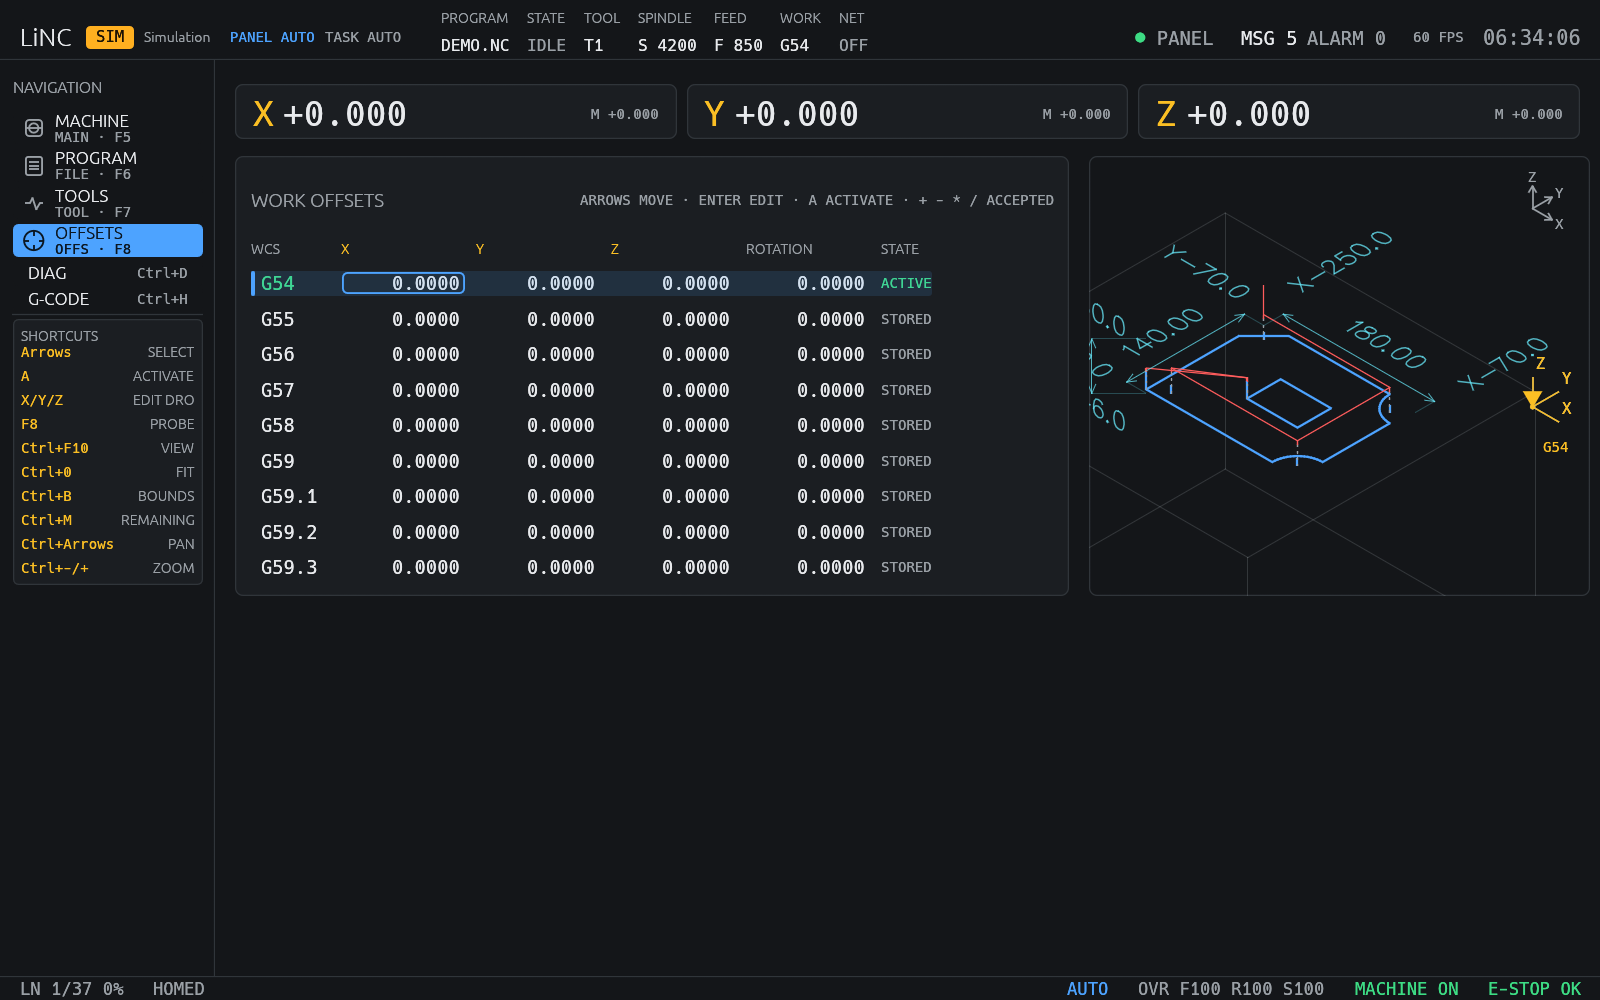
\includegraphics[width=\textwidth]{img/ui/offsets.png}
  \caption{The Offsets page: the DRO row, the nine work coordinate systems with rotation, and
           the preview drawn in machine space.}
  \label{fig:offsets}
\end{figure}

The Offsets page holds the nine work coordinate systems the controller numbers,
\texttt{G54} to \texttt{G59.3}, each with a rotation column, plus the tool offsets.

\begin{itemize}
  \item \textbf{The DRO row} shows the active system's work coordinates large, with the machine
        coordinate small underneath. A work value is edited in place and accepts arithmetic;
        committing writes the position with \texttt{G10 L20}, so the DRO reads the value you
        entered and the offset moves to match.
  \item \textbf{\keycap{A}} makes the highlighted row the active system without leaving the
        page. The controller selects it with an MDI block, and the interface verifies the
        active index it reports afterwards.
  \item \textbf{\keycap{X}}, \keycap{Y} and \keycap{Z} open the DRO for that axis.
  \item \textbf{\keycap{F8}} moves on to the probe tabs; \keycap{Esc} comes back here.
  \item \textbf{The preview} is drawn in machine space in the work system the program selects,
        so the part sits where it will be cut. The view keys work as everywhere else
        (\chordtwo{Ctrl}{F10}, \chordtwo{Ctrl}{0}, \chordtwo{Ctrl}{B},
        \chordtwo{Ctrl}{M}, \keycap{Ctrl}+arrows, \mbox{\keycap{Ctrl}+\texttt{+}/\texttt{-}}).
\end{itemize}

G92 is deliberately not exposed here. It is a transient shift that silently moves every work
system, and a field for it invited a machine state that neither the DRO nor a program could
explain.

\begin{cautionbox}
  A work offset moves the program, not the machine. The preview shows the effect before you run
  anything: check where the part sits after an edit, especially after a rotation.
\end{cautionbox}
